\documentclass[../../main.tex]{subfiles}
\graphicspath{{\subfix{../../image/}}} % 指定图片目录,后续可以直接使用图片文件名。

% 例如:
% \begin{figure}[h]
% \centering
% \includegraphics{image-01.01}
% \caption{图片标题}
% \label{fig:image-01.01}
% \end{figure}
% 注意:上述\label{}一定要放在\caption{}之后,否则引用图片序号会只会显示??.

\begin{document}

\section{群作用}

\begin{definition}[置换群(对称群)]
令 \(S\) 是一个集合,则 \(S\) 上的\textbf{置换群}(或\textbf{对称群}),记作 \((\mathrm{Perm}(S), \circ)\),由所有 \(S\) 到自身的双射构成,而这里的运算是映射的复合运算。此即
\begin{align*}
\mathrm{Perm}(S) &= \{f : S \to S \text{ 双射}\} .
\end{align*}
\end{definition}
\begin{proof}
首先,映射的复合是满足结合律的。这是根据定义立刻可知的。

单位元是恒等映射,记作 \(\mathrm{id}\),对所有 \(s \in S\),定义为
\begin{align*}
\mathrm{id}(x) &= x .
\end{align*}
故显然有,对所有 \(f \in \mathrm{Perm}(S)\),\(f \circ \mathrm{id} = \mathrm{id} \circ f = f\)。

逆元是根据双射可知的。假如 \(f\) 是一个从 \(S\) 到自身的双射,则存在其逆映射 \(f^{-1}\),使得 \(f \circ f^{-1} = f^{-1} \circ f = \mathrm{id}\)。

综上所述,\((\mathrm{Perm}(S), \circ)\) 是个群,称为 \(S\) 上的置换群(或对称群)。 
\end{proof}

\begin{example}
设 \(S = \{1, 2, \cdots, n\}\),记 \(S_n = \mathrm{Perm}(S) = \{f : S \to S \text{ 双射}\}\)。证明:\(\vert S_n \vert = n!\)。
\end{example}
\begin{proof}
设 \(f : S \to S\) 是双射,我们逐个定义 \(f\) 的像。
首先,\(f(1)\) 有 \(n\) 种不同的取法,取定 \(f(1)\) 以后,\(f(2)\) 就只有 \(n - 1\) 种不同的取法,否则 \(f(1) = f(2)\) 与双射矛盾。依此类推,可知 \(f(i)\) 就只有 \(n + 1 - i\) 种不同的取法,\(i = 1, 2, \cdots, n\)。
故 \(f\) 就有 \(n!\) 种不同的取法,即 \(\vert S_n \vert = n!\)。 
\end{proof}

\begin{proposition}
令 \((G, \cdot)\) 是一个群,我们定义 
\begin{align*}
\phi :(G,\cdot )\rightarrow (\mathrm{Perm(}G),\circ ),x\mapsto \phi _x.
\end{align*}
其中$\phi _x:G\rightarrow G,y\mapsto xy$.则 \(\phi\) 是个群同态。
\end{proposition}
\begin{proof}
证明是很简单的。令 \(x, y \in G\),对于 \(z \in G\),我们有
\begin{align*}
(\phi_x \circ \phi_y)(z) &= x(yz) = (xy)z = \phi_{xy}(z)
\end{align*}
由于这对于所有 \(z \in G\) 都成立,故
\begin{align*}
\phi_x \circ \phi_y &= \phi_{xy}
\end{align*}
即
\begin{align*}
\phi(xy) &= \phi(x) \circ \phi(y)
\end{align*}
这就证明了 \(\phi: G \to \mathrm{Perm}(G)\) 是个群同态。 
\end{proof}

\begin{definition}[群作用]
令 \((G, \cdot)\) 是一个群,$S$是一个非空集合,而 \(\phi: G \to \mathrm{Perm}(S)\)。若 \(\phi\) 是一个群同态,则我们说 \(\phi\) 是 \(G\) 在(集合)\(S\) 上的\textbf{群作用}。
\end{definition}

\begin{proposition}[群作用的等价条件]\label{proposition:群作用的等价条件}
设$G$是一个群,$S$是一个非空集合.
\begin{enumerate}[(1)]
\item 若$\phi$是 \(G\) 在 \(S\) 的群作用,记$\mathrm{Perm}\left( S \right) =\left\{ \phi _x:x\in G \right\}$,则一定满足
\begin{gather*}
\forall s\in S,e\cdot s=s,\text{即}\forall s\in S,\phi _e\left( s \right) =s.
\\
\forall x,y\in G,\forall s\in S,x\cdot (y\cdot s)=(xy)\cdot s,\text{即}\forall x,y\in G,\forall s\in S,\phi _x\left( \phi _y\left( s \right) \right) =(\phi _x\circ \phi _y)\left( s \right) =\phi _{xy}\left( s \right) .
\end{gather*}

\item 若$\phi :G\times S\rightarrow S$是满足
\begin{gather*}
\forall s\in S,e\cdot s=s,\text{即}\forall s\in S,\phi \left( e,s \right) =s.
\\
\forall x,y\in G,\forall s\in S,x\cdot (y\cdot s)=(xy)\cdot s,\text{即}\forall x,y\in G,\forall s\in S,\phi \left( x,\phi \left( y,s \right) \right) =\phi \left( xy,s \right) .
\end{gather*}
的映射,则一定存在一个\(G\) 在\(S\) 上的群作用$\widetilde{\phi }$.
\end{enumerate}
\end{proposition}
\begin{remark}
这里我们用 \(x \cdot s\),甚至 \(xs\),来代表 \(\phi_x(s)\),或 \(\phi(x, s)\)(其中 \(x \in G\),\(s \in S\)).
\end{remark}
\begin{note}
命题中的第一条性质,是说明 \(\phi\) 是良定义的(\(\phi_x\) 是双射),而第二条性质是说明 \(\phi\) 是同态。二者缺一不可。这两条性质加起来,就是群作用的定义。
\end{note}
\begin{proof}
\begin{enumerate}[(1)]
\item 若 \(\phi\) 是一个群作用,则显然利用同态的性质我们有第二条。而根据\hyperref[proposition:群同态保持逆元和单位元]{同态把单位元映到单位元},我们有 \(\phi_e = \mathrm{id}\),即对所有 \(s \in S\),\(es = s\)。这就证明了(1)。

\item 对 \(\forall x \in G\),令
\begin{gather*}
\phi_x: S \to S,  s \mapsto \phi(x, s) = xs,\\
\phi_{x^{-1}}: S \to S,  s \mapsto \phi(x^{-1}, s) = x^{-1}s.
\end{gather*}
从而由假设可知,对 \(\forall s \in S\),都有
\begin{align*}
\phi_x \circ \phi_{x^{-1}}(s) &= xx^{-1}s = es = s,\\
\phi_{x^{-1}}(s) \circ \phi_x &= x^{-1}xs = es = s.
\end{align*}
因此 \(\phi_{x^{-1}}\) 是 \(\phi_x\) 的逆映射,故对 \(\forall x \in G\),\(\phi_x\) 都是双射。于是 \(\{\phi_x : x \in G\} \subset \mathrm{Perm}(S)\)。令
\begin{gather*}
\widetilde{\phi}: G \to \mathrm{Perm}(S), x \mapsto \phi_x.
\end{gather*}
由假设可知,对 \(\forall x, y \in G\),\(\forall s \in S\),都有
\begin{align*}
x \cdot (y \cdot s) = (xy) \cdot s &\Leftrightarrow (\phi_x \circ \phi_y)(s) = \phi_{xy}(s).
\end{align*}
因此 \(\phi_{xy} = \phi_x\phi_y\),\(\forall x, y \in G\)。故 \(\widetilde{\phi}(xy) = \widetilde{\phi}(x)\widetilde{\phi}(y)\),\(\forall x, y \in G\)。即 \(\widetilde{\phi}\) 是群同态。进而 \(\widetilde{\phi}\) 就是 \(G\) 在 \(S\) 上的一个群作用。 
\end{enumerate}
\end{proof}

\begin{definition}[共轭作用]
令 \((G, \cdot)\) 是一个群,我们对 \(x \in G\),定义 \(\phi_x \in \mathrm{Perm}(G)\),对 \(y \in G\),定义为
\begin{align*}
\phi_x(y) &= xyx^{-1}.
\end{align*}
则 \(\phi: G \to \mathrm{Perm}(G)\),对 \(x \in G\),定义为 \(\phi(x) = \phi_x\),被称为 \(G\) 的\textbf{共轭作用}。 
\end{definition}

\begin{proposition}\label{proposition:共轭作用是群作用}
令 \((G, \cdot)\) 是一个群,则 \(G\) 的共轭作用是 \(G\) 在自身的一个群作用。
\end{proposition}
\begin{proof}
首先,我们要说明 \(\phi_x\) 是双射,而这是显然的,因为其逆是 \(\phi_{x^{-1}}\)。而这是因为,对于 \(y \in G\),
\begin{align*}
(\phi_x \circ \phi_{x^{-1}})(y) &= \phi_x(x^{-1}yx) = x(x^{-1}yx)x^{-1} = y\\
(\phi_{x^{-1}} \circ \phi_x)(y) &= \phi_{x^{-1}}(xyx^{-1}) = x^{-1}(xyx^{-1})x = y
\end{align*}
这样,\(\phi: G \to \mathrm{Perm}(G)\) 就是良定义的。接下来,我们证明 \(\phi\) 是个同态。令 \(x, y \in G\),\(z \in G\),则
\begin{align*}
(\phi_x \circ \phi_y)(z) &= \phi_x(yzy^{-1}) = x(yzy^{-1})x^{-1} = (xy)z(xy)^{-1} = \phi_{xy}(z)
\end{align*}
这对所有 \(z \in G\) 都成立,故
\begin{align*}
\phi_{xy} &= \phi_x \circ \phi_y
\end{align*}
即
\begin{align*}
\phi(xy) &= \phi(x) \circ \phi(y)
\end{align*}
这就证明了共轭作用确实是一个群在自身的群作用。 
\end{proof}

\begin{proposition}
令 \((G, \cdot)\) 是一个群,\(x \in G\),则 \(\phi_x: G \to G\),对 \(y \in G\),定义为
\begin{align*}
\phi_x(y) &= xyx^{-1} .
\end{align*}
是一个群 \(G\) 的自同构(即到自身的同构).
\end{proposition}
\begin{proof}
由\hyperref[proposition:共轭作用是群作用]{命题\ref{proposition:共轭作用是群作用}的证明}可知\(\phi_x\) 一定是双射,因为它的逆是 \(\phi_{x^{-1}}\)。因此我们只须证明 \(\phi_x\) 本身还是个同态(不是说 \(\phi\) 是同态,而是说每个 \(\phi_x\) 是同态)。因此我们令 \(y, z \in G\),只须证明 \(\phi_x(yz) = \phi_x(y)\phi_x(z)\)。而这是因为
\begin{align*}
\phi_x(y)\phi_x(z) &= (xyx^{-1})(xzx^{-1}) = x(yz)x^{-1} = \phi_x(yz).
\end{align*}
恰好约掉。这就证明了共轭作用下的每一个 \(\phi_x\) 都是群 \(G\) 的自同构。 
\end{proof}

\begin{definition}[内自同构与外自同构]
令 \((G, \cdot)\) 是一个群,则一个 \(G\) 的(由 \(x \in G\) 引出的)\textbf{内自同构},指的是 \(\phi_x: G \to G\),对 \(y \in G\),定义为
\begin{align*}
\phi_x(y) &= xyx^{-1}.
\end{align*}
而其他所有 \(G\) 上的自同构,则称为 \(G\) 上的\textbf{外自同构}。 
\end{definition}

\begin{definition}[轨道与稳定化子]
令 \(\phi: (G, \cdot) \to (\mathrm{Perm}(S), \circ)\) 是一个 \(G\) 在 \(S\) 的群作用。若 \(s \in S\)。则我们定义 \(s\) 的\textbf{轨道},记作 \(\mathrm{Orb}(s)\),定义为
\begin{align*}
\mathrm{Orb}(s) &= \{s' \in S : \exists x \in G, s' = xs\} = \{xs : x \in G\}.
\end{align*}
我们定义 \(s\) 的\textbf{稳定化子},记作 \(\mathrm{Stab}(s)\),定义为
\begin{align*}
\mathrm{Stab}(s) &= \{x \in G : xs = s\} .
\end{align*} 
\end{definition}

\begin{figure}[H]
\centering
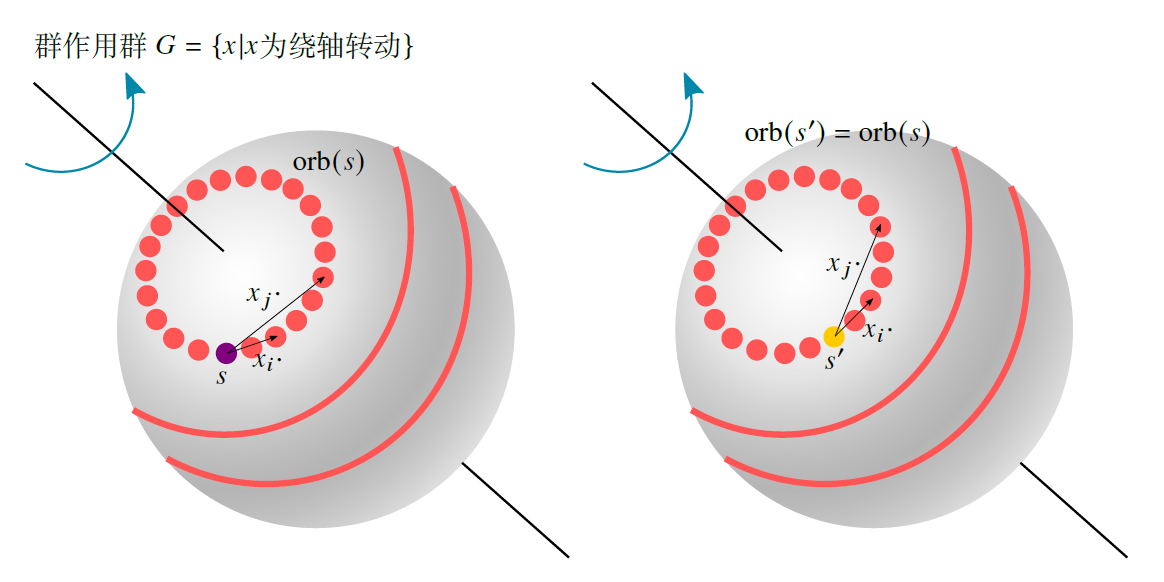
\includegraphics[scale=0.4]{群作用与轨道.png}
\caption{群作用与轨道}
\label{figure:群作用与轨道}
\end{figure}

\begin{proposition}
令 $\phi:(G,\cdot)\to(\mathrm{Perm}(S),\circ)$ 是一个 $G$ 在 $S$ 的群作用,而 $s,s'\in S$,则 $\mathrm{Orb}(s)$ 与 $\mathrm{Orb}(s')$ 要么相等,要么无交。因此,$S$ 可以写成轨道的无交并。
\end{proposition}
\begin{proof}
假设它们有交集,即假设 $s''\in\mathrm{Orb}(s)\cap\mathrm{Orb}(s')$。进一步,我们找到 $x,x'\in G$,使得 $s'' = xs = x's'$。根据对称性,我们只须证明 $\mathrm{Orb}(s)\subset\mathrm{Orb}(s')$。

任取 $ys\in\mathrm{Orb}(s)(y\in G)$,则
\begin{align*}
ys=(yx^{-1})xs=(yx^{-1})x's'=(yx^{-1}x')s'\in\mathrm{Orb}(s')
\end{align*}
根据对称性,我们就知道 $\mathrm{Orb}(s)=\mathrm{Orb}(s')$。 
\end{proof}


\begin{lemma}
令 $\phi:(G,\cdot)\to(\mathrm{Perm}(S),\circ)$ 是一个 $G$ 在 $S$ 的群作用,$s\in S$,$x,y\in G$,则 $xs = ys$ 当且仅当 $x^{-1}y\in\mathrm{Stab}(s)$。
\end{lemma}
\begin{proof}
对 $xs = ys$ 两边同时左乘 $x^{-1}$,就显然了。 
\end{proof}

\begin{theorem}[轨道 - 稳定化子定理]\label{theorem:轨道 - 稳定化子定理}
令 $\phi:(G,\cdot)\to(\mathrm{Perm}(S),\circ)$ 是一个 $G$ 在 $S$ 的群作用,$s\in S$,则存在 $G/\mathrm{Stab}(s)$ 到 $\mathrm{Orb}(s)$ 的双射。
特别地,若 $G$ 是有限群,则
\begin{align*}
|G| = |\mathrm{Stab}(s)|\cdot|\mathrm{Orb}(s)|.
\end{align*}
\end{theorem}
\begin{proof}
令 $f:G/\mathrm{Stab}(s)\to\mathrm{Orb}(s)$,定义为 $f(x\,\mathrm{Stab}(s)) = xs$。

首先证明 $f$ 是良定义的。根据上面的引理,若 $x\,\mathrm{Stab}(s)=y\,\mathrm{Stab}(s)$,则 $x^{-1}y\in\mathrm{Stab}(s)$,故 $xs = ys$。

根据 $\mathrm{Orb}(s)$ 的定义,$f$ 显然是一个满射。

单射则是再次利用上面的引理。若 $xs = ys$,则 $x^{-1}y\in\mathrm{Stab}(s)$,故 $x\,\mathrm{Stab}(s)=y\,\mathrm{Stab}(s)$。

假如 $G$ 是有限群,则同时取集合大小,就得到了
\begin{align*}
|G| = |\mathrm{Stab}(s)|\cdot|\mathrm{Orb}(s)|
\end{align*}

综上,我们就证明了轨道 - 稳定化子定理。 
\end{proof}


\begin{definition}
二面体群 $D_{2n}$,它是由所有正 $n$ 边形到自身的对称变换所构成的。

对称变换就是把自身映到自身,而且是保距的。

保距指的是,原先距离相同的点,变换后距离仍然相同。
\end{definition}
\begin{note}
如\reffigure{figure:置换群中的对称变换}中的例子. 
\begin{figure}[H]
\centering
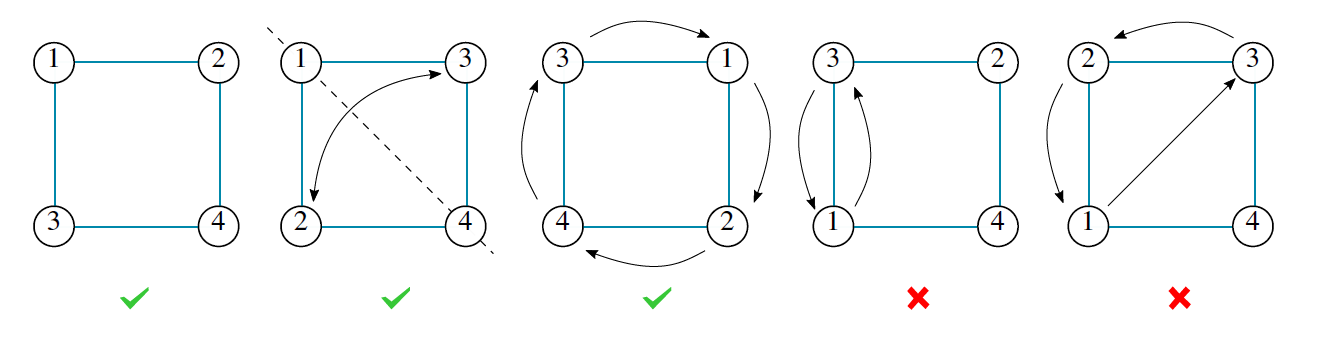
\includegraphics[scale=0.4]{置换群中的对称变换.png}
\caption{置换群中的对称变换}
\label{figure:置换群中的对称变换}
\end{figure}
\end{note}

\begin{example}
$|D_{2n}| = 2n.$
\end{example}
\begin{note}
事实上,每一个对称变换由其 $n$ 个顶点的像唯一确定,因为其余的点都可以通过顶点来找到位置。很明显,$D_{2n}$中的元素都是个轴对称图形,有 $n$ 个翻折变换;这还是个中心对称图形,有 $n$ 个旋转变换.
由此可知,二面体群 $D_{2n}$ 就是恰好由 $n$ 个翻折变换和 $n$ 个旋转变换所组成的群.
\end{note}
\begin{proof}
任取正多边形的一个顶点 $s$,考虑其轨道 $\mathrm{Orb}(s)$。最多只有 $n$ 个顶点可以去,而 $n$ 个旋转变换恰好带 $s$ 去了这些顶点,因此 $|\mathrm{Orb}(s)| = n$。

接下来,考虑其稳定化子 $\mathrm{Stab}(s)$。如果 $x\in D_{2n}$ 把 $s$ 映射到 $s$,但又有保证是一个等距变换,则 $s$ 相邻的两个顶点一定要被映射到这两个顶点。其中一个是恒等变换,而另一个是沿 $s$ 所在的对称轴的翻折变换。不难看出,这两个是唯二的 $s$ 的稳定化子。因此 $|\mathrm{Stab}(s)| = 2$。

根据\reftheorem{theorem:轨道 - 稳定化子定理},$|D_{2n}| = |\mathrm{Orb}(s)|\cdot|\mathrm{Stab}(s)| = 2n$。这就证明了这个命题。
\end{proof}




\end{document}